\documentclass[thesis.tex]{subfiles}

\begin{document}

\chapter[Experimental observations]{Experimental observation of \\single particle orientational dynamics}\label{sec:experiment}

In a collaborative project with the group of Dag Hanstorp (Gothenburg university) we develop an experimental setup for observing the orientational dynamics of single particles. The aim is to understand which mechanisms, which forces, that are crucial to include in a description of the particle dynamics. By quantitatively measuring the trajectories of individual particles, we aim to narrow down the possible choices of mechanisms driving the particle dynamics. The project has thus far resulted in Paper A of this thesis, which describes observations of both periodic and aperiodic tumbling of rod-shaped particles. At the time of this writing a round of refined experiments are ongoing, and a publication containing the results is planned.

\section{Overview \& setup}

A laboratory experiment is an idealisation of a natural system. We wish to capture and control the system, while retaining its core behaviour. So the first question is: which are the properties of the physical system we want to realise in the lab?

Since we want to study the orientational dynamics of single particles, our ideal physical system is a fluid flow, with one small, suspended particle. In particular, we would like the following features:
\begin{itemize}
	\item A known fluid flow, which does not change in time as the particle moves.
	\item A known particle geometry, so that the hydrodynamic force can be calculated.
	\item Small particles, in the sense that $\st\ll1$ and $\rep\ll1$.
	\item But not too small particles, in the sense that $\per\gg1$.
\end{itemize}
We realise this system in a tiny rectangular pipe, a microfluidic channel. Its smallest dimension is \unit[0.2]{mm}, and it is manufactured by molding plastic in a precision machined metal mold. The channel is made several centimeters long, and in each end a thin teflon tube is connected as inlet or outlet. A photograph of a channel is shown in Fig.~\ref{fig:exp_setup}. We used a mix of glycerol and water in the experiments of paper A, and the fluid is pumped through the channel with a syringe. The channel is mounted in a microscope equipped with a video camera, which in turn is connected to a computer that stores the image sequences.

The particles are plastic rods produced by stretching epoxy glue as it hardens. The rods measure around $\unit[20\textrm{-}40]{\mu m}$ in length and $\unit[1\textrm{-}2]{\mu m}$ in thickness, comparable to a single yeast cell which is around $\unit[10]{\mu m}$ in size. When we calculate the Stokes and particle Reynolds numbers for a rod in our experiment, we find that $\st \approx 10^{-6}$ and $\rep \approx 10^{-5}$, which qualifies as a small particle. We also compute the rotational Pecl\'et number and find that $\per\approx10^{4}$. Thus we realise the condition of small, but not too small particles. 

The more complicated features of our wish list are instead the fluid flow, and the particle geometry. By designing the channel to be wide and shallow we can consider the fluid flow as known. How is discussed in detail in the paper. But the exact shape of the particles remains unknown. As mentioned above, the particles are roughly rod-shaped, with a length ten times longer than its diameter. In a microscope we can easily see features of around $\unit[10]{\mu m}$, but it cannot resolve anything much smaller than $\unit[1]{\mu m}$. Resolving such small differences may seem unnecessary, but can in fact make all the difference. The observation of the effects of these small asymmetries is the main point of paper A. In the next section I will extend the discussion of this point a bit further than what is published in the paper.

\section{Results \& discussion}

In the paper we suggest, without much elaboration, that the data shown correspond to chaotic tumbling of triaxial particles. In this section I want to explain our reasons for this suggestion.

The main results presented in the paper are the trajectories of $\ve n$ shown in Figs.~6 through 8. Recall that $\ve n$ is a unit vector pointing along the axis of symmetry of the rod. From the recorded image sequences we extract $\ve n$ as function of time\footnote{Actually, we extract $\ve n(d)$, where $d$ is the distance advected along the streamline. As shown in the paper this corresponds to time $t$ when writing down for instance Jeffery's equation. This technical detail is of no importance to the present discussion.}. For an axisymmetric rod, the two degrees of freedom contained in $\ve n$ fully determines the orientation of the rod. The third degree of freedom is the rotation around the symmetry axis of the rod. Clearly, also an axisymmetric rod may rotate around its symmetry axis, but this \emph{intrinsic rotation} makes no physical difference. But in the case of an asymmetric rod the intrinsic rotation is physically relevant, and a description of the orientational dynamics must contain all three rotational degrees of freedom. In our experiment we can not resolve the intrinsic rotation, so in order to analyse the effects of asymmetry we have to figure out what its signature is in the observable $\ve n$. As I now will explain, the signature shows up in the trajectories of $n_z$, shown in panel (c) of all figures in the paper. 

For the purposes of this discussion we treat the rod as an ellipsoid. An ellipsoid has three distinct axes, and the vector $\ve n$ is attached to one of them. We introduce the third degree of freedom by an additional unit vector $\ve p$, atteched to another of the ellipsoid axes (Fig.~\ref{fig:n_p_def}). The geometry of the ellipsoid is characterised by two aspect ratios. The aspect ratio $\lambda$ is associated with the axis in the direction of $\ve n$, like in the paper. We denote the second aspect ratio $\mu$, it is associated with the axis in the direction of $\ve p$. 

In the case of axisymmetric particles, the Jeffery equation of motion for $\ve n$ is derived from a torque balance, as described in the the introduction of this thesis. In the same way we derive an equation of motion for $\ve n$ and $\ve p$ in the case of a triaxial ellipsoid. The details of this calculation are found in Appendix~\ref{app:triaxial_equation}. The equations of motion are
\begin{align}
	\diff{\ve{n}}{t} &= \ma O \ve{n} + \frac{\lambda^2-1}{\lambda^2+1} \left(\ma S \ve n- \ve{n}\transpose \ma S \ve{n})\ve{n}\right) + \frac{ 2\lambda^2 (1 - \mu^2) }{(\lambda^2+\mu^2)(\lambda^2+1)}(\ve{n}\transpose \ma S \ve{p})\ve{p} \nn\\
	\diff{\ve{p}}{t} &= \ma O \ve{p} + \frac{\mu^2-1}{\mu^2+1}\left(\ma S \ve p - \ve{p}\transpose \ma S \ve{p})\ve{p}\right) + \frac{ 2\mu^2 (1 - \lambda^2) }{(\mu^2+\lambda^2)(\mu^2+1)}(\ve{n}\transpose \ma S \ve{p})\ve{n}.\eqnlab{triaxial_equation}
\end{align}
Here, as in the introduction, $\ma S$ and $\ma O$ are the symmetric and anti-symmetric parts of the flow gradient,
\begin{align*}
	&\ma O = \frac{1}{2}(\ma A - \ma A\transpose),\quad
	\ma S = \frac{1}{2}(\ma A + \ma A\transpose),\quad
	\ma A = \nabla \ve u = \ma O + \ma S.
\end{align*}
We note the similarity between the equations for $\ve n$ and $\ve p$ in \Eqnref{triaxial_equation}. Exchanging the aspect ratios $\lambda \leftrightarrow \mu$ and the meaning of $\ve n \leftrightarrow \ve p$, must result in the same equations -- it is the same particle. Secondly, we see that the complicated coupling between $\ve n$ and $\ve p$ occurs through the strain $\ma S$. The vorticity $\ma O$ generates a simple solid-body rotation.

The action of the strain matrix $\ma S$ is to collapse both $\ve n$ and $\ve p$ onto its primary eigendirection. But the rigidity of the particle prevents this, and instead a rotation is induced. Exactly which rotation is determined by the particle shape: the strain has more influence on an elongated axis. This is especially clear in the special case where the axis in the direction of $\ve p$ is not elongated at all, that is the axisymmetric case $\mu = 1$. Then
\begin{align}
	\diff{\ve{n}}{t} &= \ma O \ve{n} + \frac{\lambda^2-1}{\lambda^2+1} \left(\ma S \ve n- \ve{n}\transpose \ma S \ve{n})\ve{n}\right) \nn\\
	\diff{\ve{p}}{t} &= \ma O \ve{p} - \frac{   \lambda^2-1 }{\lambda^2+1}(\ve{n}\transpose \ma S \ve{p})\ve{n}.\eqnlab{triaxial_equation_symm}
\end{align}
In this case we recognise the Jeffery equation for $\ve n$, without any coupling to $\ve p$. But the equation for $\ve p$ is coupled to $\ve n$.  In addition to the simple rotation of the vorticity, the action of the strain on $\ve n$ dictates the motion of $\ve p$ through the rigidity condition. As soon as an asymmetry, that is $\mu \neq 1$, is introduced, our observable quantity $\ve n$ will be influenced by $\ve p$.

We now move on to discuss the solutions of \Eqnref{triaxial_equation} in simple shear flows. For the axisymmetric case, \Eqnref{triaxial_equation_symm} admits analytical solutions for $\ve n$. The solutions, described in the introduction of this thesis, are the periodic Jeffery orbits. Two important characteristics of the Jeffery orbits are
\begin{enumerate}
	\item they describe monotonous tumbling, the vector $\ve n$ always rotates around the vorticity with positive angular velocity,
	\item the orbits are periodic, the particle always returns to its initial condition in a fixed time.
\end{enumerate}
The general triaxial case does not allow any closed form solution, and the solutions are not periodic. However, as discovered by Hinch and Leal \cite{hinch1979}, the property of monotonous tumbling still holds. That is, the vector $\ve n$ will rotate around the vorticity with a positive angular velocity. This allows us to reduce the dimensionality of the problem with a Poincar\'e surface-of-section. In practise this means that we choose a plane containing the vorticity vector, then we follow the trajectory of an initial condition on that plane until it hits the plane again. The result is a two-dimensional map, because the same initial condition will always result in the same final point. The monotonous tumbling guarantees that the trajectory always returns to the surface-of-section.

We choose as surface-of-section the plane $n_x=0$, which is when the rod is perpendicular to the flow direction. In the surface-of-section we choose the coordinates $(\psi, n_z)$. The coordinate $n_z$ is the same as shown in the results of the experiment, it is the cosine of the angle to the vorticity. For an axisymmetric rod it has the interpretation of which Jeffery orbit the rod follows. In the time series $n_z(t)$, the moments where $n_x=0$ correspond exactly to the peak height of the oscillation. The $n_z$-coordinate in the surface-of-section is therefore a quantity easily read from the experimentally observed time series. The coordinate $\psi$ is the angle of intrinsic rotation. By numerical solution of \Eqnref{triaxial_equation} we construct a plot of the Poincar\'e map by choosing an initial condition and computing a long time series. At each crossing of the surface-of-section, we plot a point at $(\psi, n_z)$.

The Poincar\'e map for an axisymmetric rod with aspect ratio $\lambda=10$ and $\mu=1$ is shown in Fig.~\ref{fig:poincareA}. It consists of only horizontal lines, each corresponding to a constant value of $n_z$, in other words each corresponding to a different Jeffery orbit. Each line is actually a torus (or a circle) since the angle $\psi$ is periodic. In fact each torus in the figure consists of many, many points from different crossings of trajectories with the surface-of-section. The dynamics is confined to stay on the torus on which it begins. In Fig.~\ref{fig:poincareA} we show examples of trajectories as successive markers on the surface-of-section, accompanied by what the experimentally observed time series $n_z(t)$ would look like. The general case is that the particle does \emph{not} return to exactly its initial position in $(\psi, n_z)$-space. The dynamics proceeds in jumps of $\Delta \psi$, and the trajectory is periodic if and only if $\pi/\Delta \psi$ is rational. Nevertheless, if we disregard the intrinsic rotation, the dynamics does appear periodic in $n_z$.

\begin{figure}
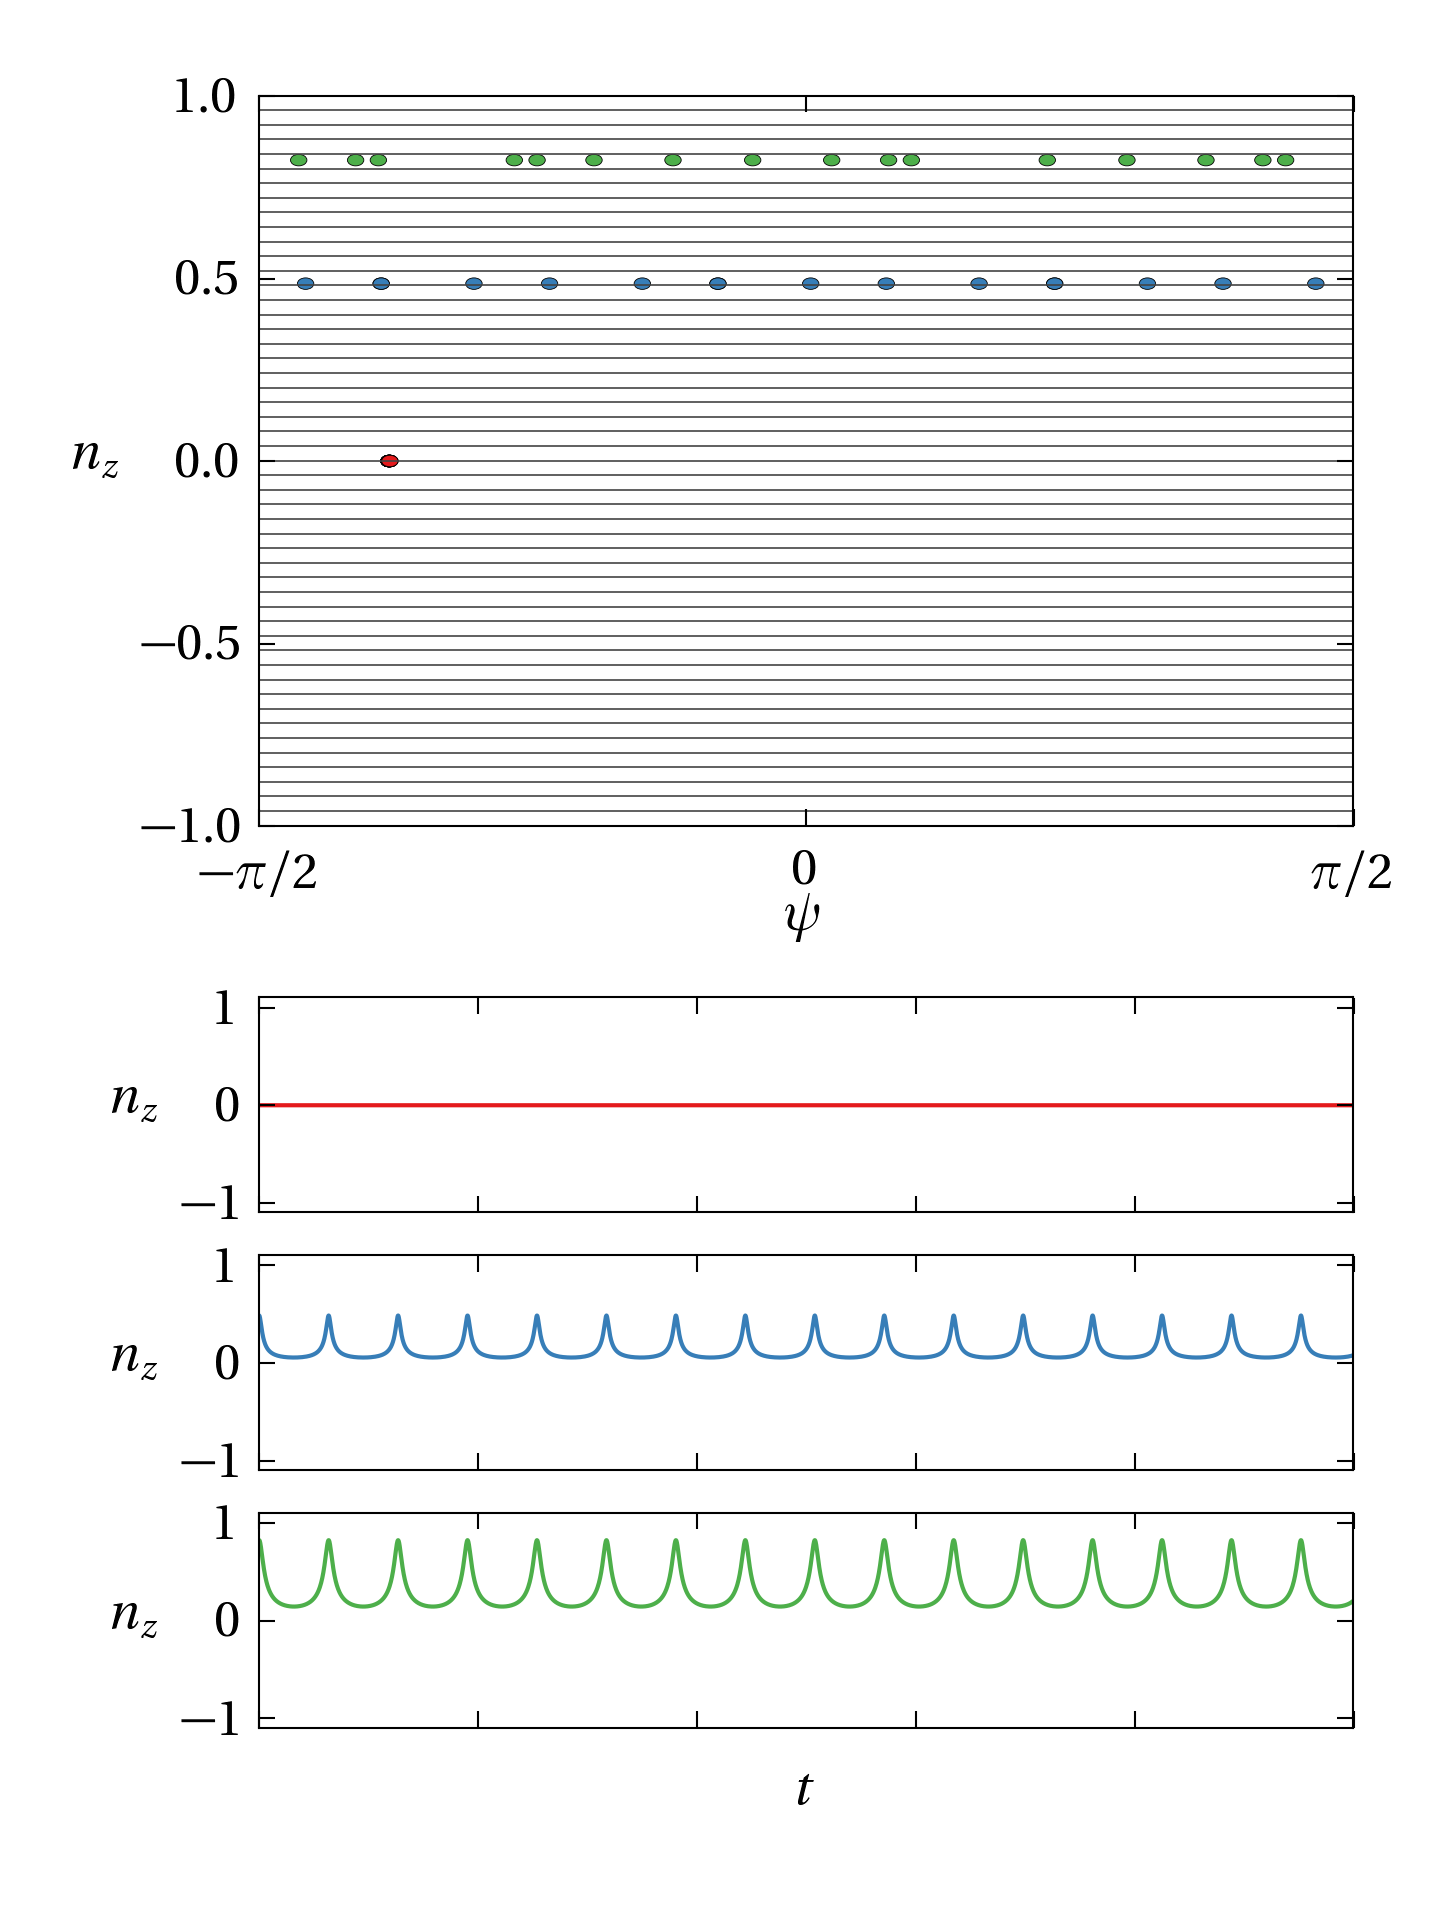
\includegraphics[width=12cm]{figs/poincareA.png}%
\caption{\label{fig:poincareA} Top: Poincar\'e surface-of-section of an axisymmetric particle with aspect ratios $\lambda=10$, $\mu=1$. Bottom: Examples of what $n_z(t)$ looks like, given the trajectory indicated by the color coded markers on the surface-of-section.}%
\end{figure}
\begin{figure}
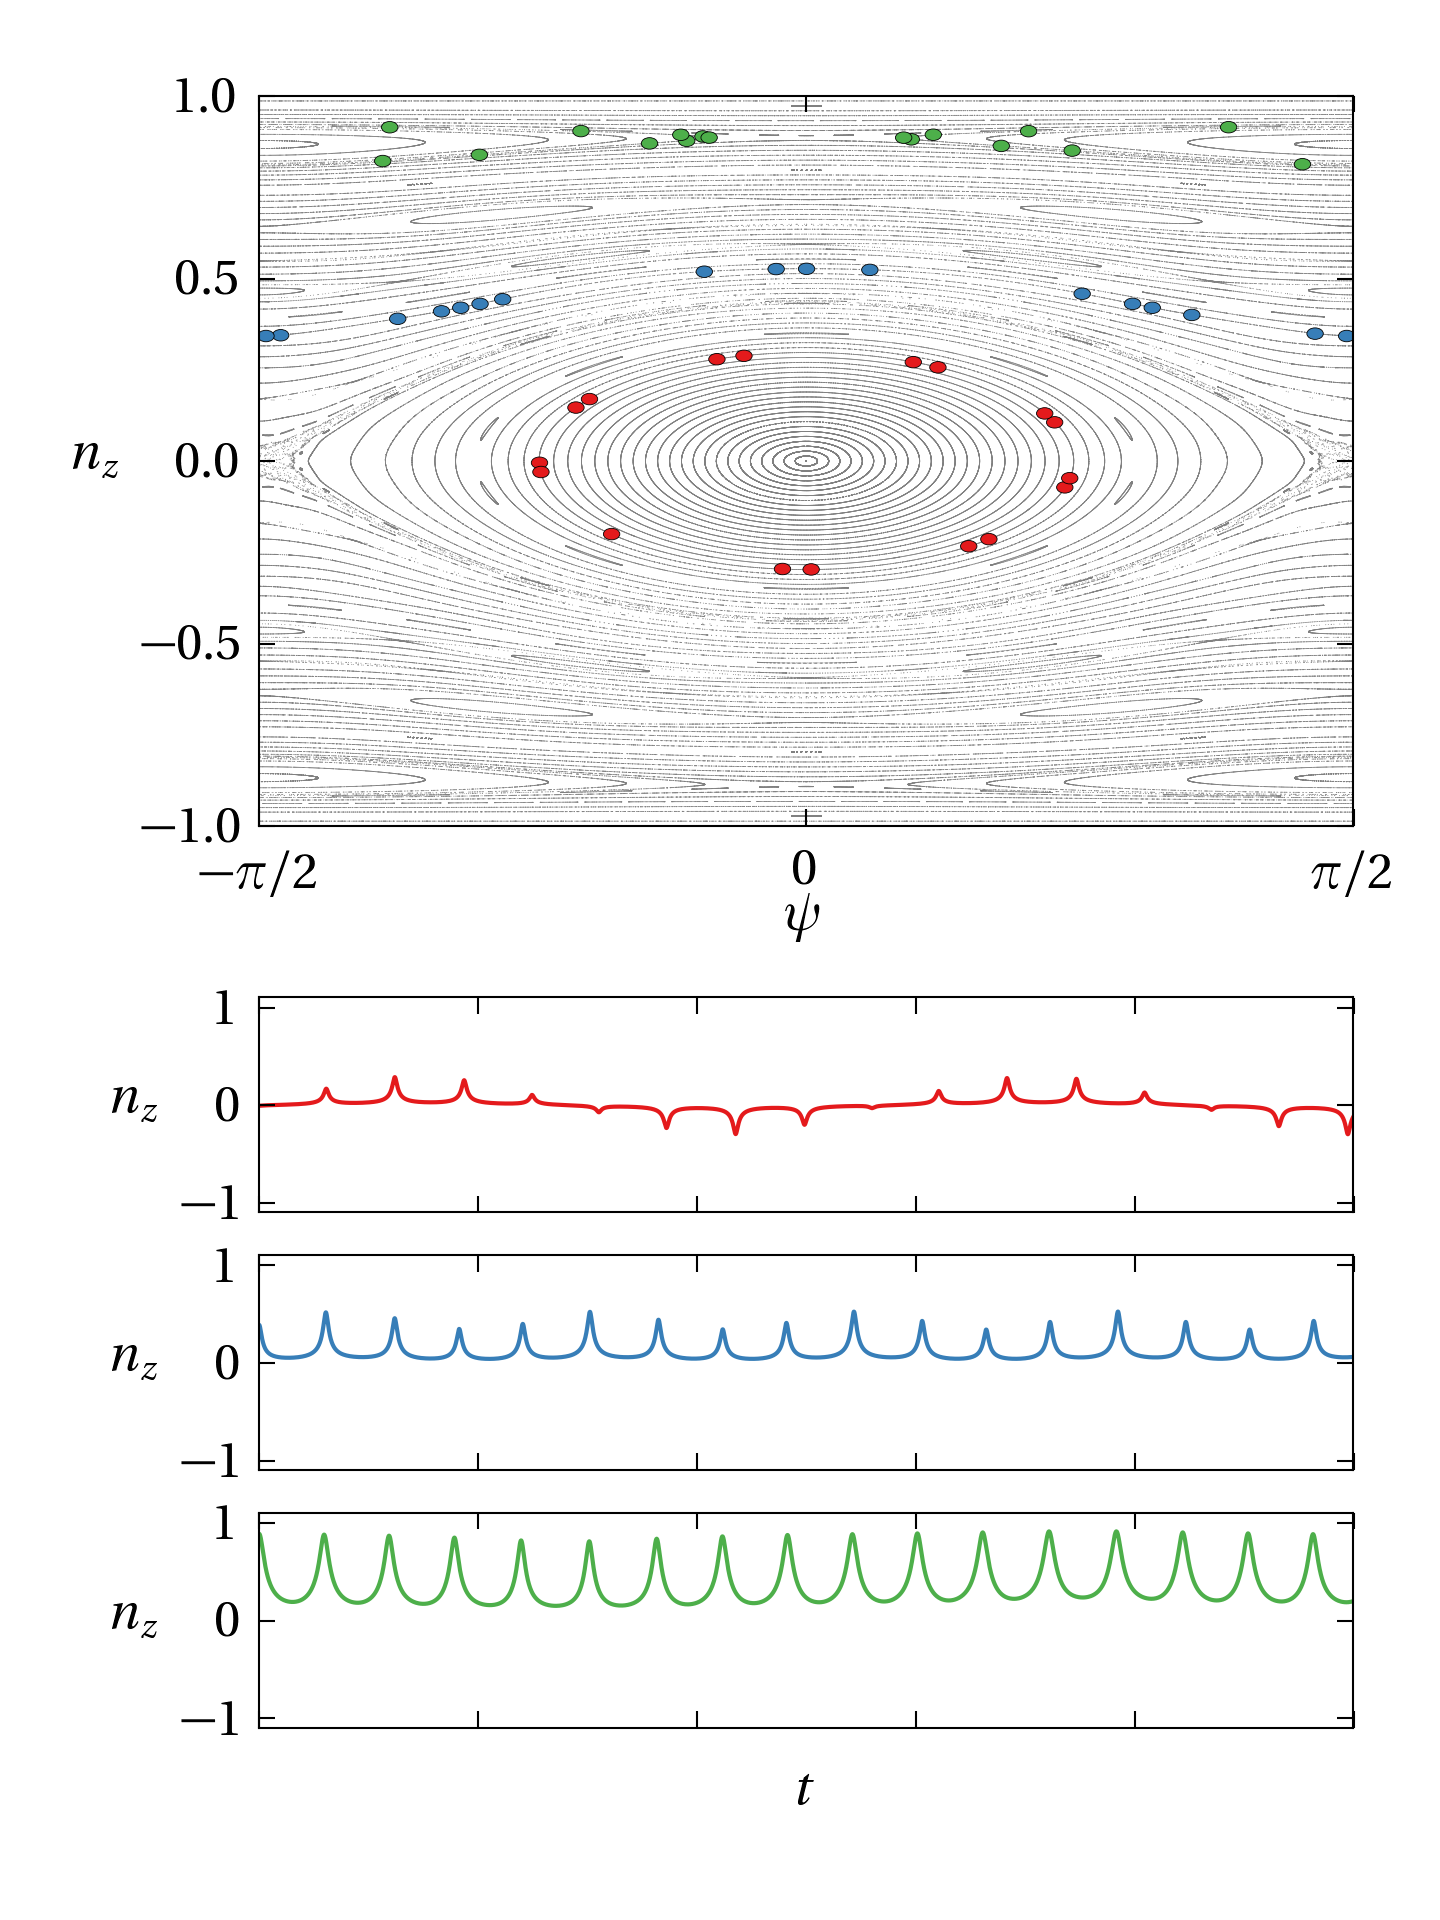
\includegraphics[width=12cm]{figs/poincareB.png}%
\caption{\label{fig:poincareB} Top: Poincar\'e surface-of-section of an asymmetric particle with aspect ratios $\lambda=10$, $\mu=1.1$. Bottom: Examples of what $n_z(t)$ looks like, given the trajectory indicated by the color coded markers on the surface-of-section. }%
\end{figure}
\begin{figure}
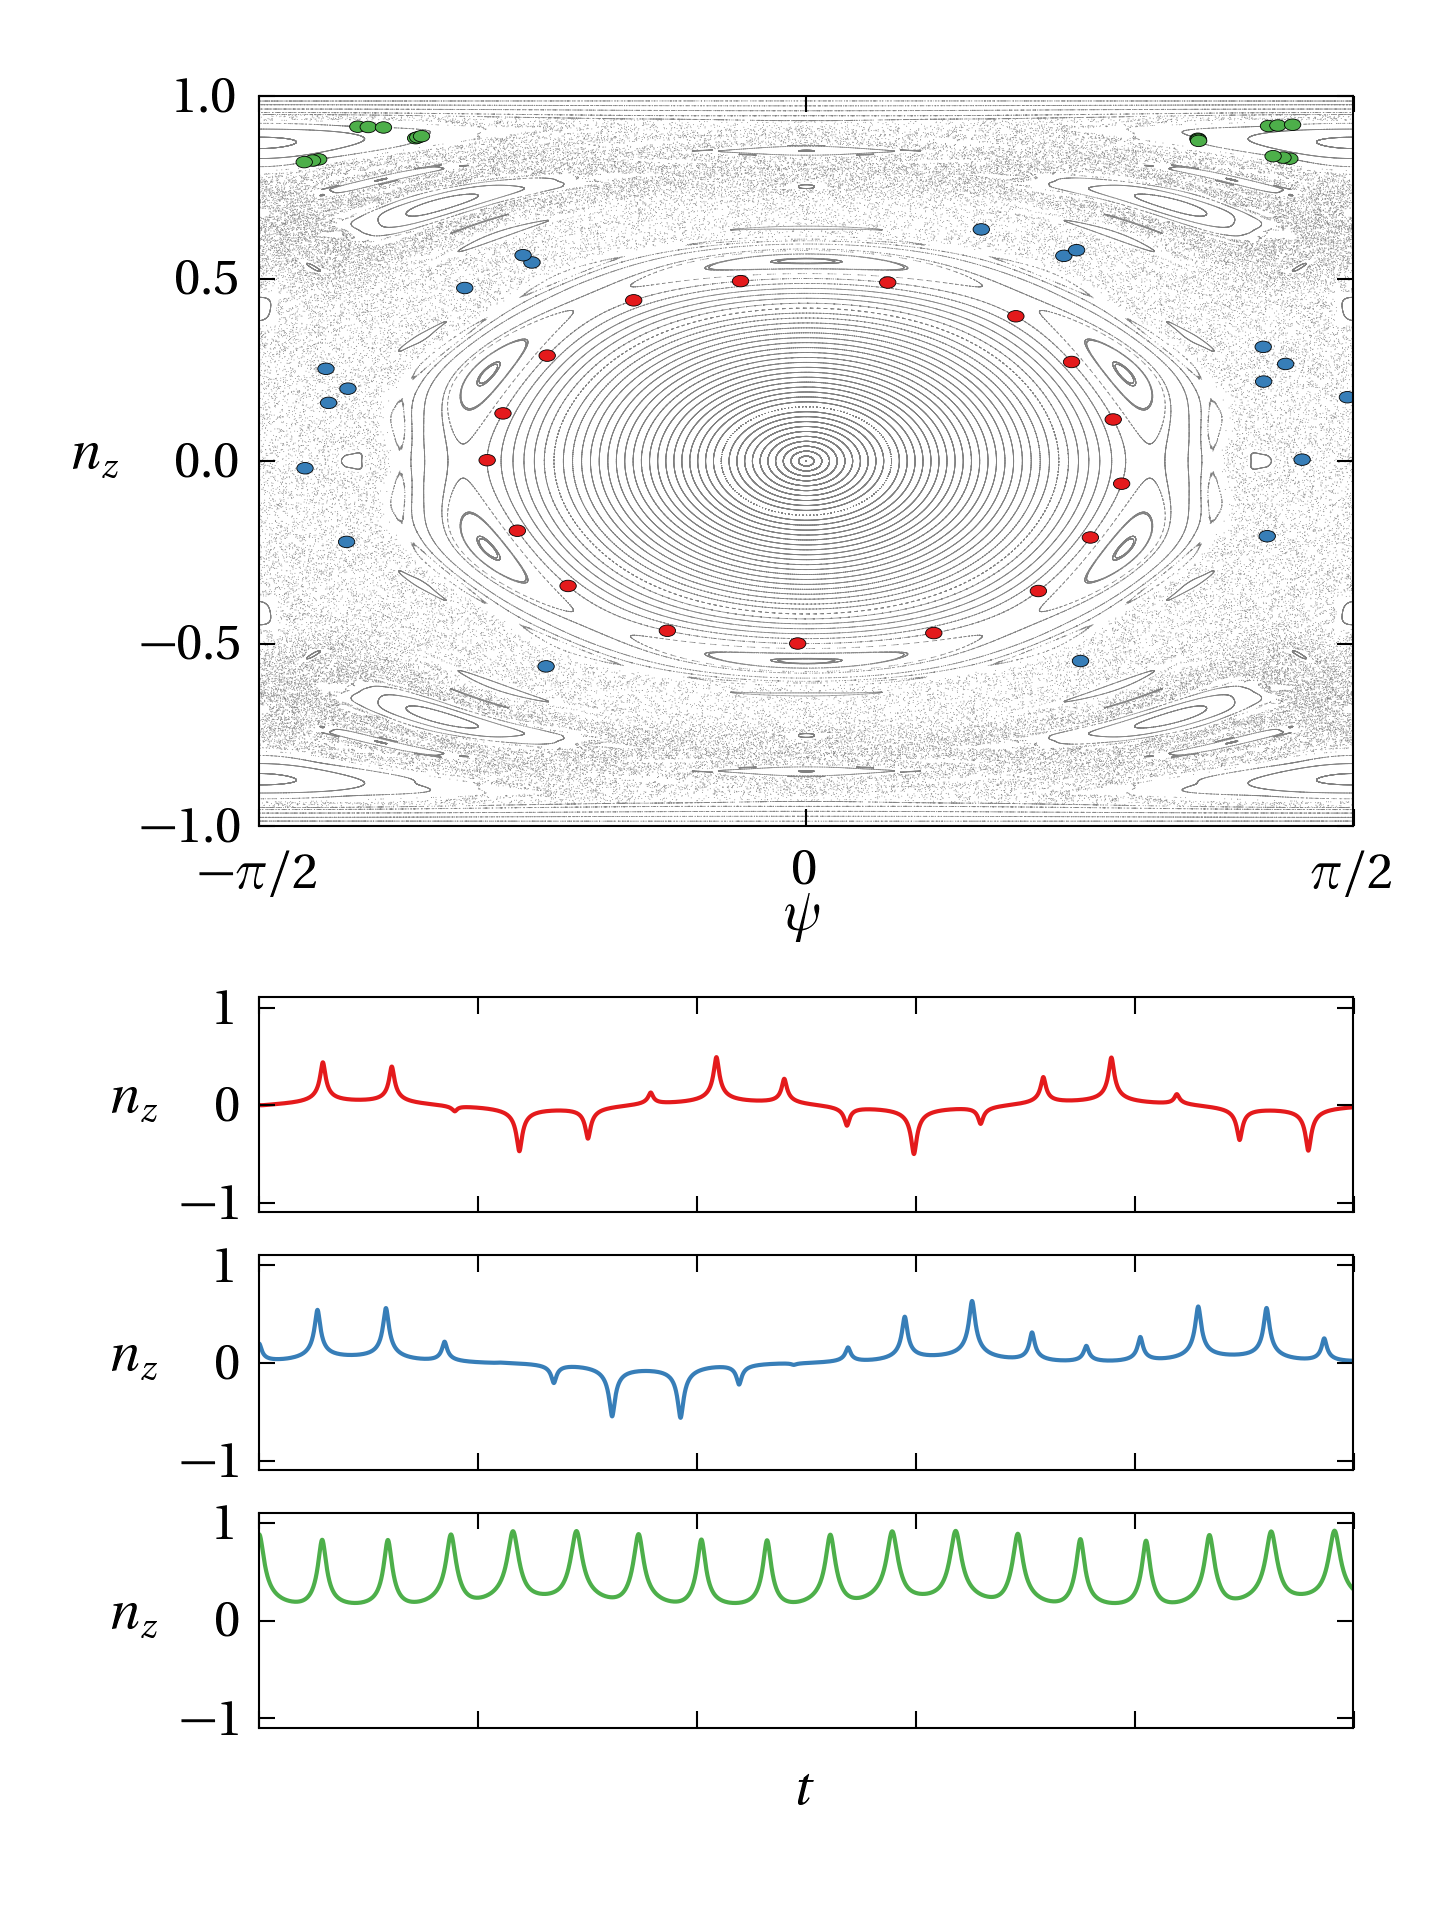
\includegraphics[width=12cm]{figs/poincareC.png}%
\caption{\label{fig:poincareC} Top: Poincar\'e surface-of-section of an axisymmetric particle with aspect ratios $\lambda=10$, $\mu=1.3$. Bottom: Examples of what $n_z(t)$ looks like, given the trajectory indicated by the color coded markers on the surface-of-section. }%
\end{figure}

In Fig.~\ref{fig:poincareB} we show the corresponding Poincar\'e map for a slightly asymmetric rod. Here $\lambda=10$ as before, but $\mu = 1.1$, that is a \unit[10]{\%} asymmetry. In the experiment this small amount of asymmetry corresponds to about $\unit[200]{nm}$ asymmetry in the particle cross-section. The effect of the asymmetry is to bend or destroy the tori. Most tori survive, but in a deformed state. Others are are broken up into a chaotic region, seen as a continuum of unordered dots in the surface-of-section. When the dynamics begins on a torus, it confined to that torus, like before. But if started in the chaotic region, it may, and will eventually, visit all parts of the chaotic region.

The picture is further distorted when we turn the asymmetry up to $\unit[20]{\%}$, as shown in Fig.~\ref{fig:poincareC}. Here the chaotic region has grown, and more tori are broken up. But it is still true that trajectories started on a torus, are confined to that torus. In the examples of $n_z(t)$ given in Figs.~\ref{fig:poincareA}-\ref{fig:poincareC} the dynamics on the torus shows up as a quasi-periodic variation. The trajectory started in the chaotic region results in a chaotic variation in $n_z(t)$.

In Paper A it is rather briefly suggested (p. 12) that the data corresponds to chaotic tumbling of a triaxial particle. I have here explained the reasons for making this suggestion. The data presented in Paper A is consistent with the trajectories in the surface-of-section, given an asymmetry of \unit[10-30]{\%}. We see regular motion, corresponding to the tori, but also chaotic motion. The tori close to $n_z=0$ are the first to break up, and are very rarely observed, while tori close to $n_z=1$ are more common. 

A complicating factor in our analysis is that each experimentally recorded trajectory corresponds to a different particle, and therefore to a different surface-of-section. Understanding this problem was key in the design the current iteration of the experiment.

\section{Outlook}

We know that each individual particle, characterised by $\lambda$ and $\mu$, has its own surface-of-section. The idea is to use a laser, an optical tweezer, to control the initial condition $n_z$ of a rod. After an experiment, the laser is used to capture the very same particle again, and reset it with a new initial condition. By repeating this procedure we can map out which tori are bent, and which are unaffected. This work is underway by Alexander Laas, a Master's thesis worker in the group.

Another important question is to consider the alternative mechanisms that could affect the particle dynamics. The effect of thermal noise has been studied by many authors for the case of axisymmetric particles. A little bit of noise invalidates the rule that a trajectory is confined to its tori, in the case of axisymmetric particle this means a Jeffery orbit. Instead there is an orientational distribution over different tori.

But the corresponding question arises also for non-axisymmetric particles. A little bit of noise allows for transport between tori, and we expect an orientational distribution to exist.

\end{document}
